\textbf{3-1} 如电图3-1-1所示，在边长为 $a$ 的等边三角形区域内有匀强磁场 $\pmb{B}$，其方向垂直纸面向外。一个边长也为 $a$ 的等边三角形导体框架ABC，在 $t = 0$ 时恰好与上述磁场区域的边界重合，尔后以周期 $T$ 绕其中心在纸面内顺时针方向匀速转动，于是在框架ABC中产生感应电流。规定电流按ABCA方向流动时电流强度取正值，反向流动时取负值。设框架ABC的电阻为 $R$。试求从 $t = 0$ 到 $t_1 = \frac{T}{6}$ 时间内的平均电流强度 $\overline{I}_1$ 和从 $t = 0$ 到 $t_2 = \frac{T}{2}$ 时间内的平均电流强度 $\overline{I}_2$。

\begin{center}
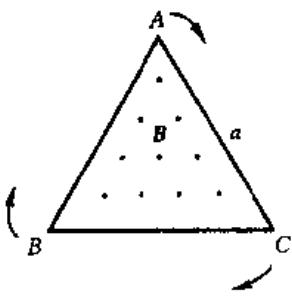
\includegraphics[width=0.2\textwidth]{figures/电图3-1-1.jpg}
\end{center}
\vfill

\textbf{3-2} 如电图3-2-1所示，ABCDA是闭合导体回路，总电阻为 $R$，$AB$ 段的一部分绕成初始半径为 $r_0$ 的圆圈。圆圈所在区域有与圆圈平面垂直的均匀磁场 $B$。回路的 $B$ 端固定，$C$ 和 $D$ 为自由端，$A$ 端在沿 $BA$ 方向的恒力 $F$ 的作用下向右移动，从而使圆圈缓慢缩小。设在圆圈缩小的过程中，始终保持圆的形状，设导体回路是柔软的，设阻力可以忽略。试求此圆圈从初始的半径 $r_{0}$ 到完全闭合所需的时间 $T$。
\begin{center}
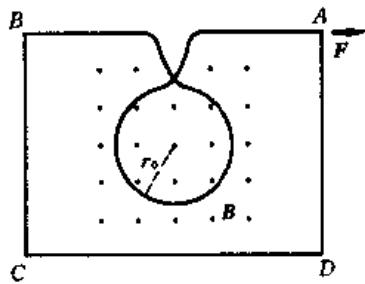
\includegraphics[width=0.2\textwidth]{figures/电图3-2-1.jpg}
\end{center}
\vfill

\newpage
\textbf{3-3} 如图3-3-1所示，铜制圆环的两个半径分别为 $r_1 = 1\,\mathrm{cm}$ 和 $r_2 = 1\,\mathrm{mm}$。圆环竖放在地面上，环底部有固定的光滑栓限制，使其不能滑动。圆环周围有竖直向上的均匀的强磁场 $B = 1.0\,\mathrm{T}$。开始时圆环偏离竖直方向一个小角度 $\theta_0 = 1.0\,\mathrm{rad}$，尔后圆环倒向地面。已知铜的电导率 $\sigma = 6.25\times 10^{7}\,(\Omega\cdot\mathrm{m})^{-1}$，质量密度 $\rho = 8.93\times 10^{3}\,\mathrm{kg/m^{3}}$。

1. 试通过数量级的估算，判断圆环倒下时其重力势能主要是转换成圆环的动能还是转换为焦耳热能。

2. 设圆环倒下过程中所受的磁力矩始终等于重力矩，试求圆环倒地所需时间 $T$。
\begin{center}
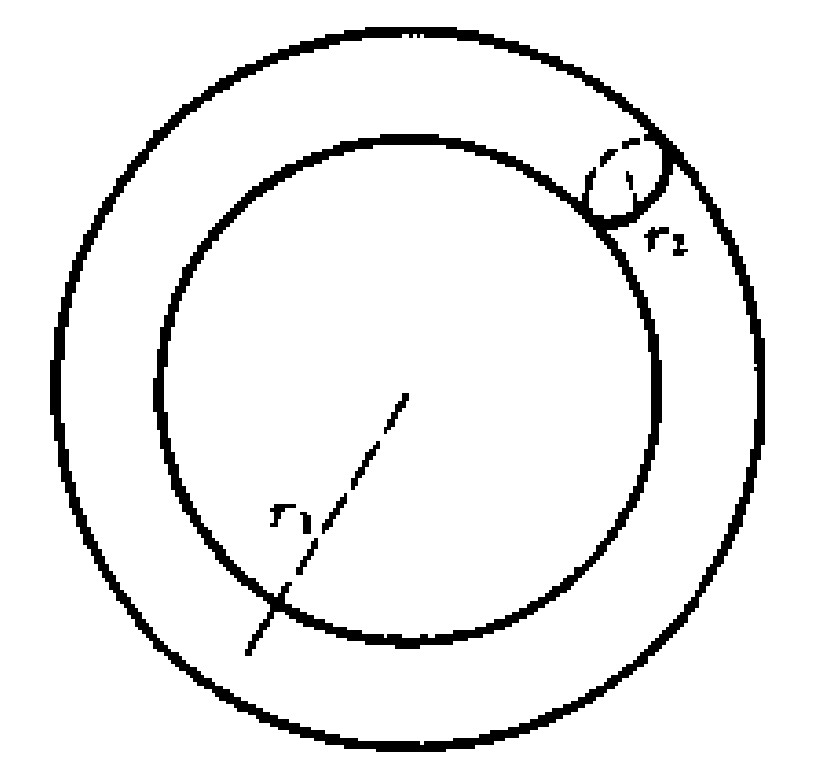
\includegraphics[width=0.18\textwidth]{figures/电图3-3-1.jpg}
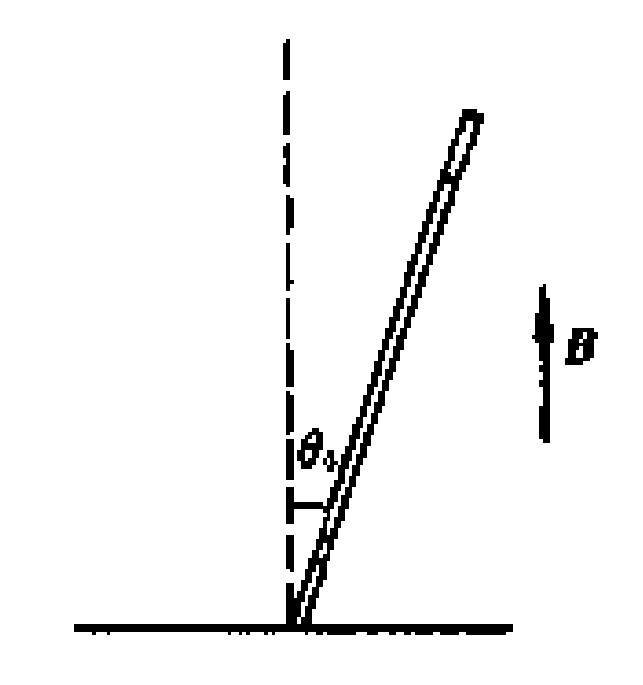
\includegraphics[width=0.18\textwidth]{figures/电图3-3-2.jpg}
\end{center}
\vfill

\textbf{3-4} 如电图3-4-1所示，在水平桌面上平放着长方形线圈abcd。已知ab边长 $l_{1}$，bc边长 $l_{2}$，线圈总电阻为 $R$，ab边正好指向北方。现将线圈以南北连线为轴翻转 $180^{\circ}$，使ab与cd边互换位置，在翻转的全过程中测得通过导线的总电量为 $Q_{1}$。然后，维持ad边（东西方向）不动，将线圈绕ad边转动 $90^{\circ}$，使之竖直，测得在竖直过程中流过导线的总电量为 $Q_{2}$。试求该处地磁场 $B$ 的大小。

\begin{center}
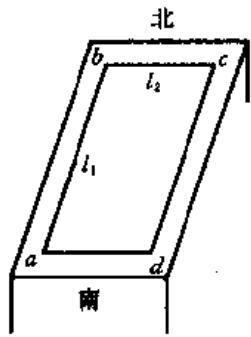
\includegraphics[width=0.15\textwidth]{figures/电图3-4-1.jpg}
\end{center}
\vfill

\newpage
\textbf{3-5} 如电图3-5-1所示为一"日"字形矩形闭合导线框。已知 $ab = bc = cd = de = ef = fa = 0.1\,\mathrm{m}$，已知 $ab, cf, de$ 段电阻均为 $3\,\Omega$，$cd, fe$ 段电阻均为 $1.5\,\Omega$，$bc, af$ 段电阻均为零。匀强磁场 $\pmb{B}$ 的方向与框面垂直向里，大小为 $B = 1\,\mathrm{T}$，磁场的边界与 $de$ 平行。今以图中向右的方向，以 $v = 24\,\mathrm{m/s}$ 的速度，将线框匀速地拉出磁场区域。试求在此过程中拉力所做的功。

\begin{center}
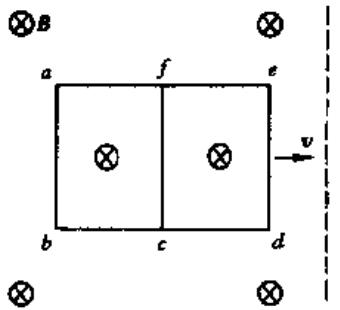
\includegraphics[width=0.2\textwidth]{figures/电图3-5-1.jpg}
\end{center}
\vfill

\textbf{3-6} 如电图3-6-1所示，在匀强磁场区域与 $\pmb{B}$ 垂直的平面（水平面）中有两根足够长的固定的平行金属导轨，在它们上面横放着两根平行导体棒，构成矩形回路。导体棒的长度均为 $l$，质量均为 $m$，电阻均为 $R$，回路中导轨部分的电阻可以忽略。设导体棒在导轨上可以无摩擦地滑行，设重力及电磁辐射均可不计，设开始时左导体棒静止，右导体棒具有向右的初速度 $v_{0}$。

试求：1. 右导体棒向右的速度 $v_{1}$ 随时间 $t$ 的变化。2. 两导体棒间距增量 $x$ 的上限。

\begin{center}
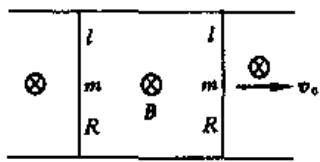
\includegraphics[width=0.25\textwidth]{figures/电图3-6-1.jpg}
\end{center}
\vfill

\newpage
\textbf{3-7} 如电图3-7-1所示，有一水平方向的匀强磁场，磁感应强度 $B$ 很大。一个半径为 $R$，厚度为 $D(D \ll R)$ 的金属圆盘，在此磁场中竖直下落，盘面始终在竖直平面内并与磁场 $\pmb{B}$ 的方向平行。设金属圆盘的电阻为零，密度为 $\rho = 9\times 10^{3}\,\mathrm{kg/m^{3}}$，所受空气阻力可略。为使圆盘在磁场中下落的加速度比没有磁场时减小千分之一，试问 $B$ 应为多大？
\begin{center}
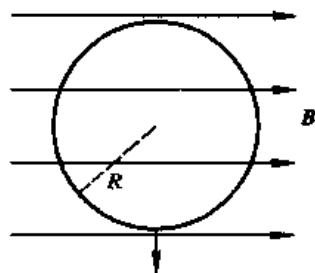
\includegraphics[width=0.2\textwidth]{figures/电图3-7-1.jpg}
\end{center}
\vfill

\textbf{3-8} 如电图3-8-1所示，宽为 $L$ 的长薄导体平板沿 $x$ 轴水平放置，平板的电阻可以忽略不计。电图3-8-1中的aebcfd为圆形均匀导线，电阻为 $3R$，圆所在平面与 $x$ 轴垂直，圆弧的两端 $a$ 和 $d$ 与导体平板的两侧边相接触，并可沿侧边自由滑动。圆弧 $ae, eb, cf, fd$ 均为 $\frac{1}{8}$ 圆周，圆弧 $bc$ 为 $\frac{1}{4}$ 圆周。一个内阻为 $R_V = nR$ 的小体积电压表位于圆心 $O$ 处，电压表的两端分别用理想导线与 $b$ 点和 $c$ 点连接。整个装置处在匀强磁场区域，$B$ 竖直向上。保持导体平板不动，圆形导线与电压表一起以恒定速度 $v$ 沿 $x$ 轴方向作平移运动。

试求：1. 电压表的读数。2. $e$ 点与 $f$ 点之间的电势差 $\Delta U_{ef}$。

\begin{center}
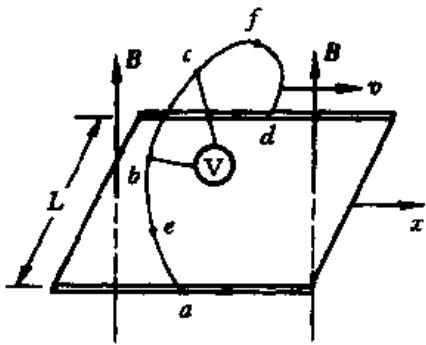
\includegraphics[width=0.2\textwidth]{figures/电图3-8-1.jpg}
\end{center}
\vfill

\newpage
\textbf{3-9} 如电图3-9-1所示,水平与垂直的两根长直导体棒相交,连接成固定不动的十字架形状．由边长为 a 的四根导体棒构成的正方形框架，从电图 3-9-1 中的实线框架位置开始，以速率 v 匀速向左运动，在运动过程中框架始终与十字架接触．空间有均匀磁场 B，其方向如电图 3-9-1，垂直于十字架和框架所在的平面．设所有导体棒单位长度的电阻为 $r=100\ \Omega/m, a=0.1\ m, v=0.24\ m/s, B=10^{-4}\ T$ .

取正方形框架在电图3-9-1中实线位置时为 $t = 0$ 时刻. 当它向左移动时将有电流 $I$ 通过十字架的垂直棒, 并且为了维持框架匀速左移, 需有适当的向左的力 $F$ 作用于框架.

1. 试求电流随时间的变化 $I(t)$ , 并画出相应的曲线。

2. 试计算在全过程中流过垂直棒的总电量 Q。

3. 试求 $F(t)$ , 并画出对应的曲线。
\begin{center}
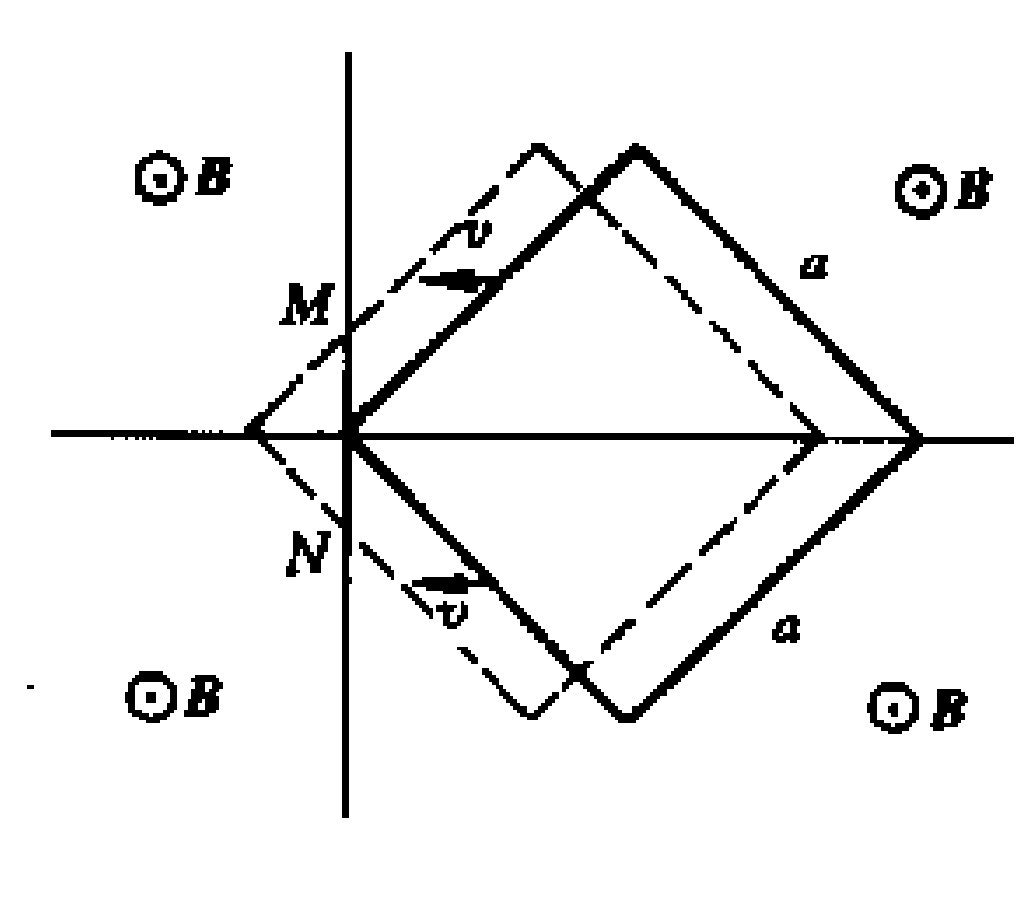
\includegraphics[width=0.2\textwidth]{figures/电图3-9-1.jpg}
\end{center}
\vfill

\textbf{3-10} 磁流体发电机的工作原理如电图3-10-1所示。横截面为矩形的管道长为 $l$，宽为 $a$，高为 $b$，上、下两个侧面是绝缘体，相距为 $a$ 的两个侧面是电阻可略的导体，这两个侧面与负载电阻 $R_{L}$ 相连。整个管道处于匀强磁场区域，$B$ 垂直于上、下侧面指向上。管道内沿长度方向流有电阻率为 $\rho$ 的电离气体，气体流速处处相同，所受摩擦阻力的大小与流速成正比。今在管的两端维持恒定的压强差 $P$，无磁场存在时气体的流速为 $v_{0}$。试求有磁场存在时，此发电机的电动势 $\mathcal{E}$。
\begin{center}
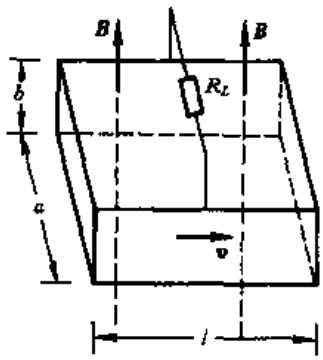
\includegraphics[width=0.15\textwidth]{figures/电图3-10-1.jpg}
\end{center}
\vfill

\newpage
\textbf{3-11} 如电图3-11-1所示，转轮1和转轮2的边缘都是很薄的良导体，每一个转轮都有四根轮辐，每根轮辐的长度为 $l$，电阻为 $r$。两轮都可绕各自的轮轴转动，两轮的边缘通过电刷用导线连接，两轮轴亦通过电刷用导线连接。整个装置放在磁感应强度为 $\pmb{B}$ 的匀强磁场中，$\pmb{B}$ 的方向垂直纸面向里。转轮2的边缘与一阻力闸A接触，开始时转轮1以角速度 $\omega_{1}$ 旋转，转轮2不动，尔后使转轮1保持其旋转角速度 $\omega_{1}$，这将使转轮2被带动并最后达到稳定的转动。设电刷与导线的电阻均可忽略不计，电刷的阻力也可忽略。设阻力闸A与转轮2之间的阻力恒为 $F$。

试求：

1. 转轮2稳定转动时的角速度 $\omega_{2}$。

2. 保持转轮1以恒定角速度 $\omega_{1}$ 转动所需的外加功率 $P$。

\begin{center}
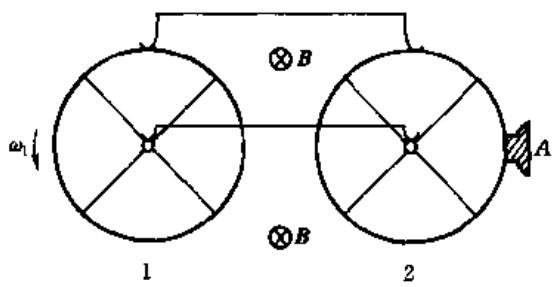
\includegraphics[width=0.2\textwidth]{figures/电图3-11-1.jpg}
\end{center}
\vfill

\textbf{3-12} 如电图3-12-1所示，由匀质细导线弯成的半径为 $a$ 的圆线圈和一内接等边三角形电阻丝构成的电路，电路中各段电阻值已在电图3-12-1中标明。在圆线圈所在平面内有垂直纸面向里的匀强磁场 $\pmb{B}$，$B$ 随时间 $t$ 均匀地减小，其变化率的大小为已知常量 $k$，设 $2r_1 = 3r_2$。试求电图3-12-1中 $A, B$ 两点之间的电势差 $U_{AB}$。

\begin{center}
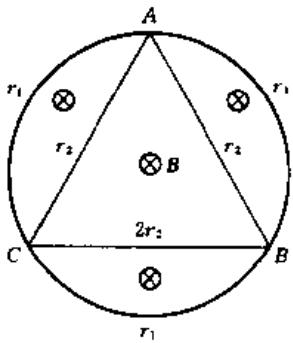
\includegraphics[width=0.18\textwidth]{figures/电图3-12-1.jpg}
\end{center}
\vfill

\newpage
\textbf{3-13} 如电图3-13-1所示，一圆柱形金属块放在高频感应炉中加热。设感应炉的线圈产生的磁场是均匀的，磁感应强度的方均根值为 $B$，频率为 $f$。金属圆柱的直径为 $D$，高为 $h$，电导率为 $\sigma$，圆柱的轴与磁场平行。设涡电流产生的磁场可以忽略。试证明在金属圆柱内因涡电流产生的平均热功率为
$$
P = \frac{\pi^{2}}{32} f^{2} B^{2} \sigma D^{4} h
$$
\begin{center}
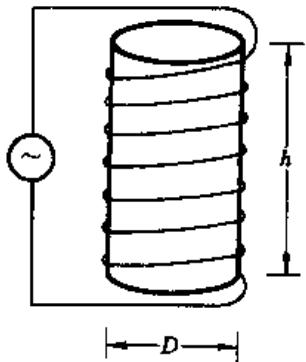
\includegraphics[width=0.18\textwidth]{figures/电图3-13-1.jpg}
\end{center}
\vfill

\textbf{3-14} 长为 $2\pi a$，电阻为 $r$ 的均匀细导线首尾相接形成一个半径为 $a$ 的圆。现将电阻为 $R$ 的伏特计，以及电阻可以忽略的导线，按电图3-14-1和电图3-14-2所示的方式分别与圆的两点相连接。这两点之间的弧线所对圆心角为 $\theta$。若在垂直圆平面的方向上有均匀变化的匀强磁场，已知磁感应强度的变化率为 $\dot{B}$。试问在电图3-14-1和电图3-14-2两种情形，伏特计的读数各为多少。

\begin{center}
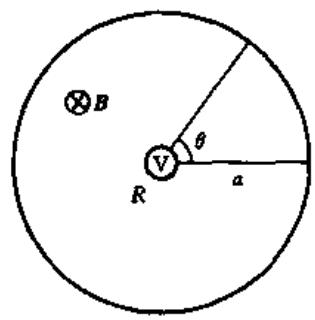
\includegraphics[width=0.18\textwidth]{figures/电图3-14-1.jpg}
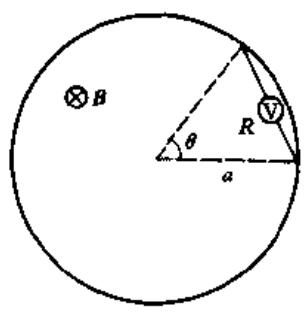
\includegraphics[width=0.18\textwidth]{figures/电图3-14-2.jpg}
\end{center}
\vfill

\newpage
\textbf{3-15} 如电图3-15-1所示，在半径为 $R$ 的无限长圆柱形区域内有匀强磁场，磁场 $\pmb{B}$ 的方向与圆柱的轴平行，垂直纸平面向外。将半径也是 $R$ 的光滑绝缘细环固定在纸平面上，并正好套住磁场区。在细环上串有一个质量为 $m$，电量为 $q(q > 0)$ 的带电小珠。设 $t = 0$ 时，磁场 $B = 0$，小珠在环上静止；$0 < t < T$ 时，$B$ 随时间 $t$ 均匀地增长；$t = T$ 时，$B = B_0$；$t > T$ 时，$B = B_0$ 不变。试定量地讨论 $t > 0$ 时小珠的运动状态及小珠对圆环的正压力（沿径向）。设纸平面为水平面，小珠所受重力与圆环支持力抵消。

\begin{center}
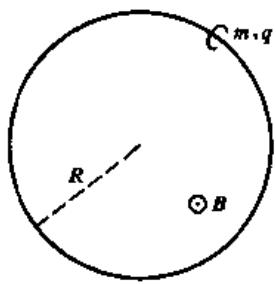
\includegraphics[width=0.18\textwidth]{figures/电图3-15-1.jpg}
\end{center}
\vfill

\textbf{3-16} 如电图3-16-1所示，在一个半径为 $r$，质量为 $m$，可以无摩擦地自由转动的匀质绝缘圆盘中部装有一细长螺线管，其半径为 $A$，沿轴线方向单位长度上绕有 $n$ 匝线圈，线圈中通以稳恒电流 $I$。在圆盘的边缘上均匀地嵌着 $N$ 个带等量正电荷 $q$ 的小球。设开始时，螺线管中的电流为 $I$，圆盘静止，然后将电流切断。试求圆盘转动的角速度。
\begin{center}
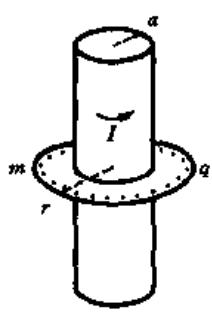
\includegraphics[width=0.15\textwidth]{figures/电图3-16-1.jpg}
\end{center}
\vfill

\newpage
\textbf{3-17} 如电图3-17-1所示，一圆柱形区域内的匀强磁场 $\pmb{B}$ 随时间 $t$ 变化，在磁场区域内垂直于 $\pmb{B}$ 的 $Oxy$ 平面上有一光滑绝缘的细空心管MN，它固定在 $x$ 轴上并相对 $y$ 轴对称。$\mathrm{MO'}$ 与 $OO'$ 之间的夹角为 $\theta_{0}$，其中 $O'$ 是磁场区域中央轴与 $xy$ 平面的交点。在管MN内有一质量为 $m$，电量为 $q(q>0)$ 的光滑小球。$t=0$ 时小球静止在M位置。设 $B$ 的方向如图所示，其大小随 $t$ 的变化规律为 $B=B_{0}\sin\omega t$，其中 $B_{0}$ 和 $\omega$ 均为正的常量。设 $B$ 的这种变化规律刚好能使小球在MN之间以 $O$ 为中心，以MN长度之半为振幅作简谐振动。

1. 试确定小球简谐振动的圆频率 $\omega_{\text{球}}$ 与 $m, q, \theta_0, B_0$ 之间的关系。

2. 设MN长为 $2R$。试求管MN受到小球作用力的 $y$ 分量 $N_y$ 与小球位置 $x$ 之间的函数关系，画出 $N_y(x)$ 曲线，并标出曲线上的特征点。

\begin{center}
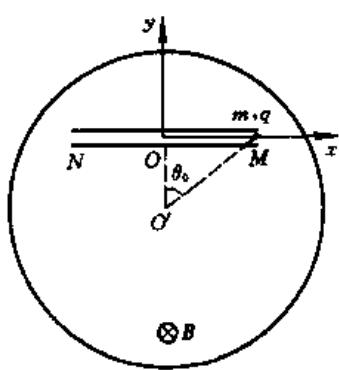
\includegraphics[width=0.15\textwidth]{figures/电图3-17-1.jpg}
\end{center}
\vfill

\textbf{3-18} 如电图3-18-1所示，在光滑的水平面上，有边长为 $l = 0.8\,\mathrm{m}$ 的正方形导线框，其质量 $m = 100\,\mathrm{g}$，自感 $L = 10^{-3}\,\mathrm{V\cdot s/A}$，电阻可忽略不计。在 $t = 0$ 时，线框右侧 $bc$ 边所在位置刚好是匀强磁场区域的左边界，磁场区域的宽度为 $s = 0.2\,\mathrm{m}$，$B$ 的方向垂直纸面向里，$B = 0.5\,\mathrm{T}$。取 $t = 0$ 时 $bc$ 边所在位置为坐标原点 $O$，取 $x$ 轴与 $bc$ 边垂直。导线框以沿 $x$ 轴正方向的初速 $v_{0}$ 运动。忽略空气阻力。

1. 设 $v_0 = 4\,\mathrm{m/s}$，试求 $t = \frac{\pi}{36}\,\mathrm{s}$ 时刻，$bc$ 边所在的位置 $x_c$。

2. 设 $v_0 = \frac{16}{\sqrt{3}}\,\mathrm{m/s}$，试求 $t = \frac{\pi}{36}\,\mathrm{s}$ 时刻 $bc$ 边所在的位置 $x_c$。
\begin{center}
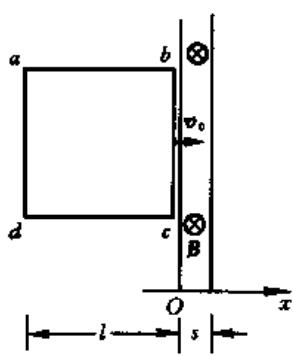
\includegraphics[width=0.15\textwidth]{figures/电图3-18-1.jpg}
\end{center}
\vfill

\newpage
\textbf{3-19} 由半径为 $1\,\mathrm{mm}$ 的导线构成的半径为 $10\,\mathrm{cm}$ 的圆形线圈处于超导状态。开始时，线圈内通有 $100\,\mathrm{A}$ 的电流。一年后测出线圈内电流的减小量不足 $10^{-6}\,\mathrm{A}$，试粗略估算此线圈电阻率的上限。
\vfill

\textbf{3-20} 如电图3-20-1所示，两根半径均为 $a = 1\,\mathrm{cm}$ 的长直圆柱形导线平行放置，两导线中央轴之间的距离为 $d = 20\,\mathrm{cm}$，在两导线中有电流强度均为 $I = 20\,\mathrm{A}$ 的反向恒定电流。

1. 试求两导线之间每单位长度的自感系数。

2. 若将两导线保持平行地缓慢分开到相距 $d' = 40\,\mathrm{cm}$。试求磁场对单位长度导线所作的功。

3. 试问移动后两导线单位长度的自感磁能改变了多少？是增加还是减少？试说明能量的来源或去向。
\begin{center}
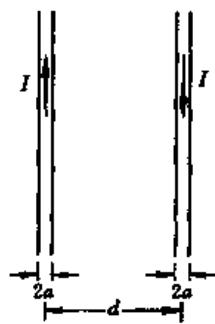
\includegraphics[width=0.15\textwidth]{figures/电图3-20-1.jpg}
\end{center}
\vfill

\newpage
\textbf{3-21} 一种磁位计的结构如电图3-21-1所示。在一条非磁性材料做的细软带上，均匀密绕着线圈，线圈的两端接在冲击电流计上。把磁位计放在某磁场中，突然把产生磁场的电流切断，使 $\pmb{H}$ 迅速变为零，由冲击电流计测出整个过程中迁移的电量为 $q$，即可得出原来的磁场沿软带的磁位降。试证明，原来磁场从软带一端的 $a$ 点沿软带到另一端 $b$ 点的磁位降为
$$
\int_{(l)^{a}}^{b} \boldsymbol{H}_{0} \cdot \mathrm{d}l = \frac{Rq}{\mu_{0}Sn}
$$

\begin{center}
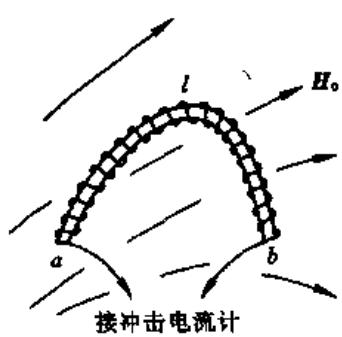
\includegraphics[width=0.15\textwidth]{figures/电图3-21-1.jpg}
\end{center}
\vfill

\textbf{3-22} 如电图3-22-1所示，两根无限长直载流导线互相平行，相距 $2a$，两导线中的电流彼此反向，电流强度相同。在两平行长直导线所在的平面内有一半径为 $a$ 的圆环，圆环刚好在两平行长直导线之间并且彼此绝缘。试求圆环与两平行长直导线之间的互感系数。

\begin{center}
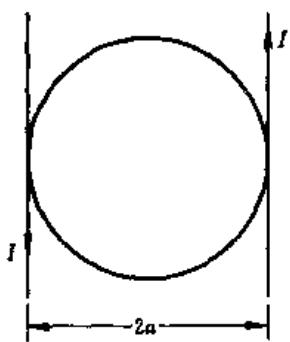
\includegraphics[width=0.15\textwidth]{figures/电图3-22-1.jpg}
\end{center}
\vfill

\newpage
\textbf{3-23} 两个载流线圈彼此很靠近，则一个线圈中的电流变化会在另一个线圈中产生感生电动势。衡量载流线圈之间这种作用的物理量是互感系数 $M$，当第一个和第二个线圈中的电流强度分别为 $I_{1}(t)$ 和 $I_{2}(t)$ 时，在第一和第二线圈中产生的感生电动势分别为 $\pm M \frac{\mathrm{d} I_{2}(t)}{\mathrm{d} t}$ 和 $\pm M \frac{\mathrm{d} I_{1}(t)}{\mathrm{d} t}$，感生电动势的符号由楞次定律确定。

根据以上说明，试计算电图3-23-1系统的等效电感 $L_{AB}$。如果使一个线圈反向缠绕，结果是否会变化，怎样变化？互感系数 $M$ 的最大值是多少？

试再计算电图3-23-2和电图3-23-3两个系统的等效电感 $L_{AB}$。如果使电感为 $L_{1}$ 的线圈反向缠绕，结果如何？

\begin{center}
    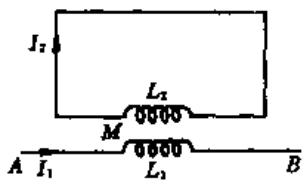
\includegraphics[width=0.3\textwidth]{figures/电图3-23-1.jpg}
    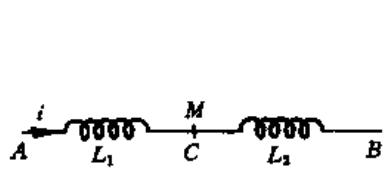
\includegraphics[width=0.3\textwidth]{figures/电图3-23-2.jpg}
    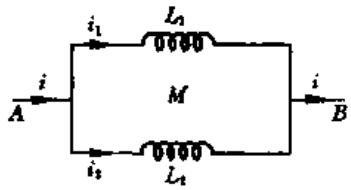
\includegraphics[width=0.3\textwidth]{figures/电图3-23-3.jpg}
\end{center}
\vfill
